\chapter{Аналитическая часть}

В данном разделе будет проанализирована предметная область и выделены её основные сущности и ограничения значений их атрибутов.
Также будет выбран тип базы данных.

\section{Анализ предметной области}

Техническое задание к данной работе предполагает создание базы данных для погодного приложения.
Следовательно, необходимо проанализировать предметную область метеорологии для выделения сущностей и связей между ними, а также атрибутов данных сущностей.

\subsection{Cущности в метеорологии}
Главной задачей метеорологии является прогнозирование погоды~[2].
Тогда основной сущностью исследуемой предметной области является погода.
Она определяется для какого-либо дня или часа.
Причём день представляется датой, а час -- временем относительно начала соответствующего дня.
Следовательно, день и час являются атрибутами погоды, а не отдельными сущностями.
Если погода определена для будущего времени, то она является прогнозом.
Поэтому нет смысла выделять прогноз как отдельную сущность.

Важной особенностью погоды является локальность.
Это значит, что она всегда ассоциируется с определённым географическим местом.
В сервисах, предоставляющих информацию о погоде, в качестве такого места рассматривается город~[4]~[5].
Тогда город -- следующая сущность предметной области.

Таким образом, к сущностям предметной области метеорологии относятся погода и город.

Далее рассмотрены составляющие погоды, представляющие интерес для пользователей её прогнозов~[1]. 
Их список:
\begin{itemize}
    \item температура воздуха;
    \item атмосферное давление;
    \item скорость ветра;
    \item относительная влажность воздуха;
    \item видимость;
    \item облачность;
    \item осадки;
    \item гроза;
    \item туман;
    \item метель;
    \item пыльные бури;
    \item гололёд.
\end{itemize}
Ещё один часто выделяемый параметр погоды -- ощущаемая температура~[4]~[5].
Он нужен для субъективного понимания пользователем текущей погоды.
Перечисленные параметры, в зависимости от способа формализации, могут быть как числовыми, так и логическими, и являются атрибутами погоды.

\subsection{Формализация сущностей предметной области}
В данном разделе будут формализованы сущности погоды и города.
Для формализации понятия погоды необходимо выделить набор формальных параметров погоды на основе выделенных её составляющих.
Для этого проанализированы существующие погодные сервисы: Яндекс Погода~[4], AccuWeather~[5], Погода <<Mail.ru>>~[6], The Weather Channel~[7].
Такие параметры погоды, как температура, давление, влажность и скорость ветра являются числовыми и измеряются в градусах по Цельсию, миллиметрах ртутного столба, процентах и метрах в секунду соответственно.
Видимость характеризуется максимальным расстоянием, на котором человек может что-либо увидеть и измеряется в километрах.
Погодные сервисы следят за двумя видами осадков: дождевыми и снежными и измеряют их в миллиметрах.
Таким образом, осадки формально описываются двумя числами: количеством выпавшего дождя и снега в миллиметрах.
Далее рассмотрены параметры погоды, не поддающиеся численному описанию.
К ним относится облачность и наличие каких-либо особых природных явлений.
Облачность представляется перечислением и чаще всего имеет следующие виды: солнечно, облачно с прояснениями, пасмурно.
Природные явления также задаются перечислением: гроза, дождь, туман, солнце, снег и метель.
Таким образом, удобно ввести тип погоды -- перечисление, которое будет содержать информацию как об облачности, так и о природных явлениях.
Оно будет включать следующие значения:
\begin{itemize}
    \item гроза;
    \item морось;
    \item дождь;
    \item ливень;
    \item туман;
    \item солнце;
    \item облачно с прояснениями;
    \item пасмурно;
    \item снег;
    \item метель.
\end{itemize}
Таким образом, пользователь сможет легко интерпретировать погоду.

Необходимо также выделить параметры такой сущности как город.
Он характеризуется названием, географическим расположением и названием страны.
Под географическим расположением подразумевается широта и долгота, выраженные в вещественных числах~[3].

Далее рассмотрены сущности, относящиеся ко времени.
День описывается датой, которая содержит год, месяц и день.
Час в прогнозе почасовой погоды всегда привязан к определённому дню и указывается порядковым номером относительно его начала.

Таким образом, все сущности предметной области метеорологии выделены и формализованы.

\subsection{Граничные значения параметров сущностей}
После описания сущностей предметной области необходимо представить требования к их целостности.
Далее представлены таблицы~\ref{table:weather_parameters}--\ref{table:city_parameters}, содержащие требования к числовым параметрам погоды и города.

\clearpage
\begin{table}[h!]
    \centering
    \begin{tabular}{ |c|c|c| }
        \hline
            \textbf{Параметр погоды} & \textbf{Ограничения} & \textbf{Единицы измерения} \\
        \hline
            температура & $-273$ -- $\infty$ & \textdegree C \\
        \hline
            ощущаемая температура & $-273$ -- $\infty$ & \textdegree C \\
        \hline
            скорость ветра & $0$ -- $\infty$ & м/с \\
        \hline
            давление & $0$ -- $\infty$ & мм рт. ст. \\
        \hline
            относительная влажность & $0$ -- $100$ & \% \\
        \hline
            дождевые осадки & $0$ -- $\infty$ & мм \\
        \hline
            снежные осадки & $0$ -- $\infty$ & мм \\
        \hline
            время восхода & $00:00$ -- $23:59$ & 24ч-формат \\
        \hline
            время заката & $00:00$ -- $23:59$ & 24ч-формат \\
        \hline
    \end{tabular}
    \caption{\centering Параметры погоды, их единицы измерения и граничные значения}
    \label{table:weather_parameters}
\end{table}

\begin{table}[h!]
    \centering
    \begin{tabular}{ |c|c|c| }
        \hline
            \textbf{Параметр города} & \textbf{Ограничения} & \textbf{Единицы измерения} \\
        \hline
            название & от 1 символа & --- \\
        \hline
            широта & $-90$ -- $90$ & градусы \\
        \hline
            долгота & $-180$ -- $180$ & градусы \\
        \hline
    \end{tabular}
    \caption{\centering Параметры города, их единицы измерения и граничные значения}
    \label{table:city_parameters}
\end{table}

\section{Требования к базе данных}
Для проектирования базы данных необходимо определить набор требований к ней.
Выделены следующие критерии для выбора типа базы данных:
\begin{itemize}
    \item наличие возможности обеспечить безопасность данных (К0);
    \item наличие возможности отслеживания целостности данных (К1);
    \item наличие возможности сжатия данных (К2);
    \item наличие возможности ускорения доступа к данным с помощью их индексации (К3);
    \item наличие возможности хранить отношения многие-ко-многим (К4);
    \item наличие возможности дешёвой разработки и сопровождения (К5).
\end{itemize}

Важным критерием (К5) является техническая возможность не только разработки, но и недорогого сопровождения.
Необходимо формализовать данный критерий, так как он субъективен.
Цена разработки пропорциональна её времени, которое зависит от наличия документации для используемых технологий.
Также на цену влияет поддерживаемость на различных операционных системах, так как если приложение и базу данных нужно будет перенести на другую ОС, то может потребоваться использование других технологий, что затрудняет разработку.
Приведённые факторы формирования цены напрямую зависят от популярности технологий, используемых при создании программного обеспечения.
Таким образом, критерий <<К5>> можно формализовать как то, что используемый тип баз данных реализован в виде технологии, являющейся одной из самых популярных или поддерживающейся одной из самых больших IT-компаний.

База данных должна предоставлять достаточно возможностей чтобы хранить все необходимые приложению сущности и связи между ними.
На рисунке~\ref{fig:er-chen} представлена диаграмма сущность-связь.
\begin{figure}[H]
	\centering
	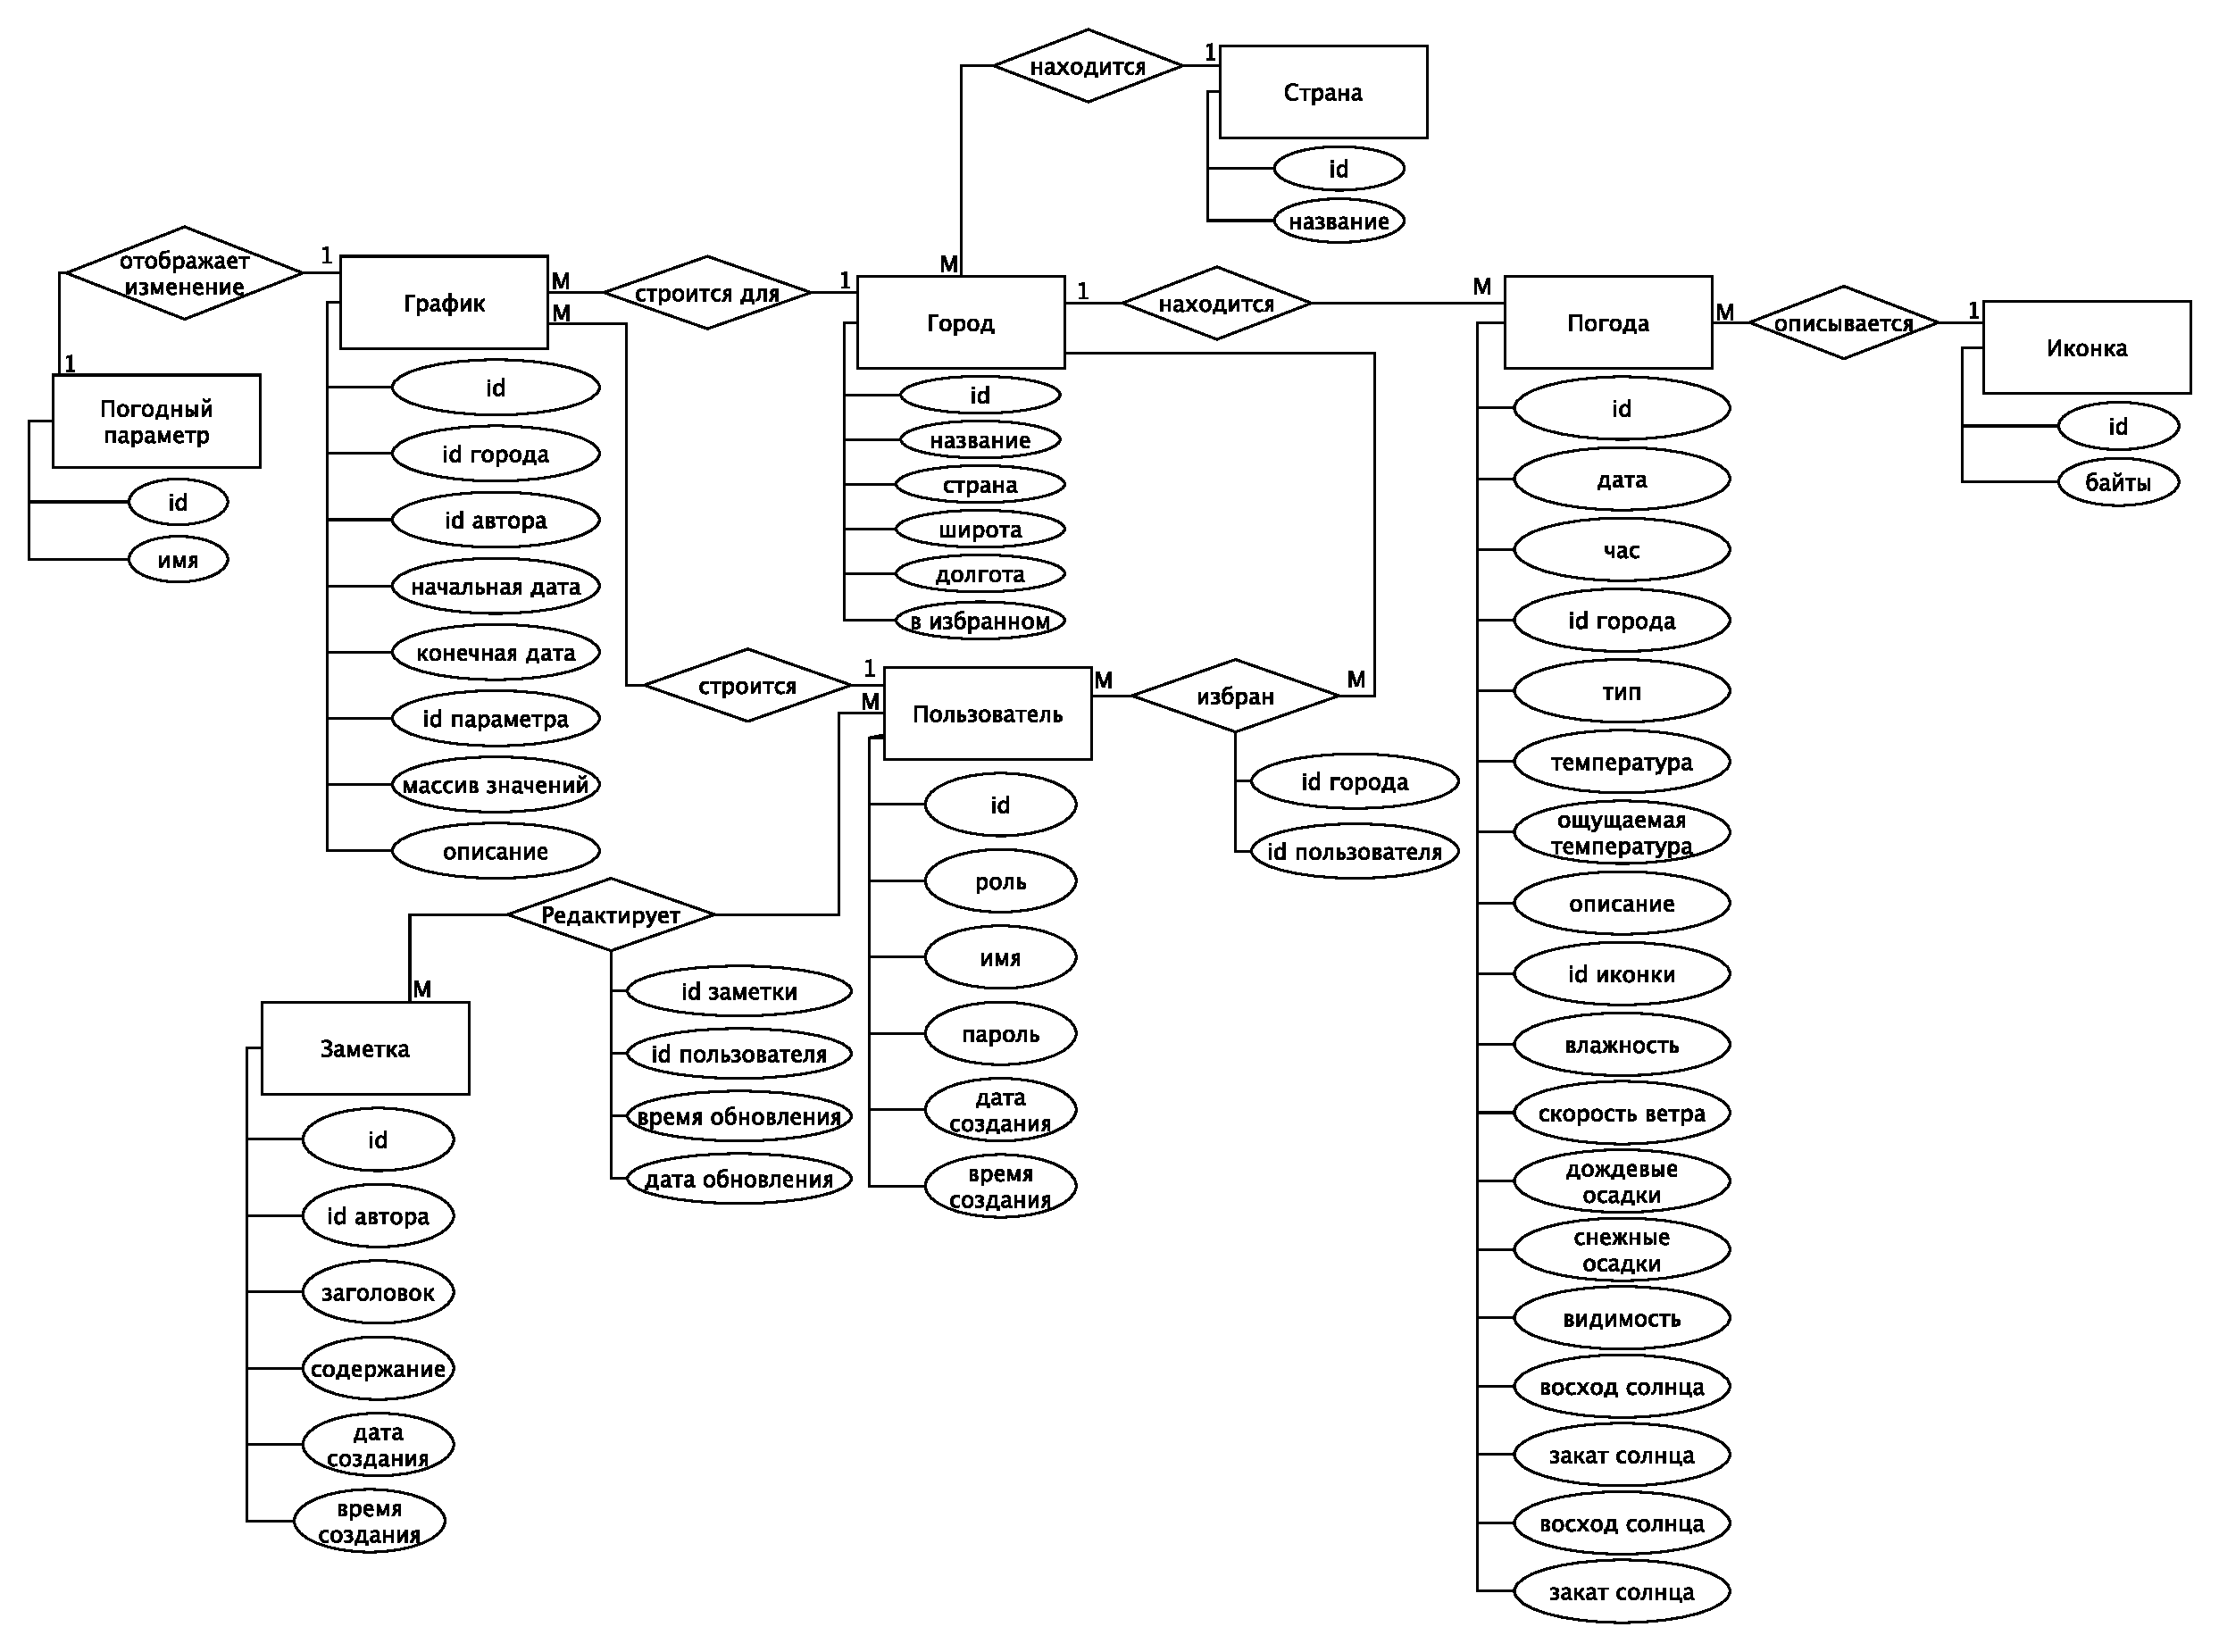
\includegraphics[height=0.55\textheight, width=\textwidth]{tools/img/er-chen.pdf}
	\caption{
        ER-диаграмма разрабатываемой базы данных в нотации Чена
    }
	\label{fig:er-chen}
\end{figure}

Другим важным требованием является удалённое хранение сущностей пользователей.
Это обеспечит возможность авторизации на другом устройстве.

\section{Выбор типа базы данных}
Существуют различные типы баз данных.
От типа зависит способ хранения информации и алгоритмы доступа к ней.
Каждый тип баз данных имеет некоторые особенности, которые могут иметь ключевое значение для удовлетворения выделенным требованиям.
Базы данных разделены на группы по модели представления данных и способу доступа к ним~[10].

К способам доступа к данным относятся~[10]:
\begin{itemize}
    \item клиент-серверный;
    \item файл-серверный;
    \item встраиваемый.
\end{itemize}
Важным замечанием является то, что файл-серверная модель доступа не обеспечивает надёжной защиты данных по определению, поэтому не будет рассматриваться из-за нарушения критерия К0.
Другое требование, предъявленных к базе данных -- удалённое хранение данных о пользователях.
Это можно сделать с помощью клиент-серверной модели взаимодействия.
Остальные сущности лучше хранить локально, так как нет необходимости публикации этих данных для совместного использования на нескольких устройствах.

К основным типам баз данных относительно модели представления информации относятся~[10]:
\begin{itemize}
    \item реляционные;
    \item документальные;
    \item графовые;
    \item встраиваемые.
\end{itemize}

Далее представлена таблица~\ref{table:cmp_model}, отображающая результаты сравнения моделей представления данных.
\begin{table}[h!]
    \centering
    \begin{tabular} { |c|c|c|c|c|c|c| }
        \hline
        \hspace{0pt} & \multicolumn{6}{|c|}{Критерий} \\
        \hline
        Тип базы данных & К0 & К1 & К2 & К3 & К4 & К5 \\
        \hline
        Реляционная & + & + & + & + & + & + \\
        \hline
        Документальная & + & - & + & + & + & + \\
        \hline
        Графовая & + & + & + & + & + & - \\
        \hline
        \end{tabular}
    \caption{\centering Параметры погоды, их единицы измерения и граничные значения}
    \label{table:cmp_model}
\end{table}
Реляционная база данных является самой популярной для решения практических задач~[8], а также, в отличие от остальных, поддерживает стандартный язык запросов -- SQL, который можно использовать на всех ОС.
Таким образом, реляционная база данных удовлетворяет критерию <<К5>>.
Документальные базы данных существуют на всех популярных ОС, таких как Android, IOS, Linux, Windows, macOS.
Также данный тип баз данных реализован в виде технологии Firebase, поддерживаемой компанией Google~[13].
Поэтому документальные базы данных удовлетворяют критерию <<К5>>.

В результате сравнения типов баз данных, целесообразно выбрать реляционную базу данных для локального хранения и документальную базу данных Firebase от Google для удалённого хранения данных о пользователях.

\section*{Выводы из аналитической части}
В данном разделе была проанализирована предметная область метеорологии, в результате чего определены её основные сущности, а также атрибуты погоды и их граничные значения.
Затем определены требования к разрабатываемой базе данных и проведён анализ существующих, в результате чего сделан выбор типа базы данных.
Таким образом, получены все необходимые сведения для проектирования.